\documentclass{llncs}
%
\usepackage{makeidx}  % allows for indexgeneration
\usepackage{graphicx}

\usepackage{algorithm}
\usepackage{algpseudocode}
\usepackage{amssymb}
\usepackage{etoolbox}
\usepackage{color}
\usepackage{changepage}
\usepackage{csquotes}
\usepackage{tabularx,booktabs,multirow}
\usepackage{longtable}
\usepackage{framed}

\graphicspath{{Graphics/}}

\newcommand{\sym}[1]{\ensuremath{\mathcal{#1}}}
\newcommand{\svm}{SVM$^{rank}$}

\setlength{\tabcolsep}{6pt}

\begin{document}

\title{Learning Constraints and Optimization Criteria}
\author{Samuel Kolb\inst{1}}
\authorrunning{Samuel Kolb} % abbreviated author list (for running head)
%%%% list of authors for the TOC (use if author list has to be modified)
\tocauthor{Samuel Kolb}
\institute{KULeuven, Leuven, Belgium}
\email{samuel.kolb@me.com}

\maketitle              % typeset the title of the contribution

\begin{abstract}
This research presents two systems that are able to automatically learn constraints from examples and optimization criteria from rankings, respectively.
Both hard and soft constraints can be learned and constraints are represented as first order logical clauses.
Choosing such clauses as representations enables the use of ILP techniques such as clausal discovery.
In this research optimization criteria are represented as weighted clauses.
For all examples, the clause learning system could find the essential constraints efficiently.
The learning system for optimization criteria is shown to achieve accurate results and can learn criteria that identify the correct optimal solution even for few examples and noisy rankings.
Finally, a procedure is outlined that allows weighted first order logic clauses to be used for optimization.
\end{abstract}

\section{Introduction {\color{red} To be shortened}}
People use computers to solve complex problems, which are hard to solve by hand.
Traditionally, programs or algorithms are written to tell the computer \emph{how} to solve a particular problem.
These programs are essentially precise, step-by-step instructions.
Alternatively, problems can be described \emph{declaratively} by formulating them in a high level language.
Such a language describes a problem without specifying how a solution is to be found.
Generic programs, called solvers, are used to find solutions to problems formulated in this language.

A popular movement within declarative programming is constraint programming.
In constraint programming users specify variables, their domains and constraints that act upon these variables.
The constraint solver assigns values to the variables such that all the constraints hold.
This solver has a large degree of freedom in choosing a search strategy and ideally the user does not need to be familiar with the underlying algorithms.

Aside from being popular in academia, it is also being used in industrial applications\cite{Simonis:IndustrialApplicationsCP}.
Much of the research on constraint programming is focused on improving solvers.
In practice, however, it can be challenging for non-experts to formulate constraints to describe their problem\cite{Wallace:PrinciplesCP}.

The first goal of this research is to automate the step of modeling a problem, in order to, amongst others, make constraint solving more accessible.
In this approach a few examples of what a user considers valid solutions are used by a computer system to find constraints.
These constraints can then be used by an existing constraint solver.

Constraints are represented as logical clauses.
This allows the use of techniques from the field of Inductive Logic Programming (ILP).
Specifically, a new implementation of the Clausal Discovery algorithm\cite{DeRaedt:ClausalDiscovery} is used.
Research on constraint learning is often done independently of ILP.
By exploiting the parallels between both fields, this research follows the same approach as Lallouet et al.\cite{Lallouet:LearningCP}.
\\\\
Hard constraints are used to distinguish solutions to a problem.
So called soft constraints can be used to express properties which do not have to be fulfilled by every solution.
Weights can be assigned to such soft constraints to express their importance.
Such weighted soft constraints can be used as optimization criteria.
Optimal solution are found by maximizing the sum of the weights of soft constraints that are fulfilled by the solution.

The second goal of this research is to learn from user preference and to formulate corresponding optimization criteria.
Using rankings over a few examples, weighted soft constraints are found.
Both the learning of constraints as the learning of optimization criteria aim to bridge the gap between problems and their formal representation.

The use of weighted soft constraints is inspired by the research of Campigotto et al.\cite{campigotto2011active}, amongst others.
Their work examines attempts to obtain similar results in an interactive context for propositional constraints.
In this research first-order logical clauses will be used.
\\\\
The weighted clauses cannot be directly used in a constraint solver.
Therefore, an approach is outlined that describes how these constraints can be used in the IDP system to obtain an optimal solution in practice.

\section{Background}
In this section a brief overview of the important concepts and relevant literature will be provided

\subsection{Clauses}
First-order logical clauses consist of a disjunction of literals.
Literals are defined as being either an atoms or a negated atom.
Clauses are often expressed using a body and a head: $\mathit{head} \leftarrow \mathit{body}$.
All literals containing a negation are grouped in the body and the other literals form the head of the clause.
\begin{eqnarray*}
  \lnot a_1 \lor \lnot a_2 \lor a_3 \lor a_4 = a_3, a_4 \leftarrow a_1, a_2 
\end{eqnarray*}

Atoms are logical concepts that can be assigned a truth value.
In this paper atoms will be restricted to either the symbols $\mathit{true}$ or $\mathit{false}$ or predicates.
Predicates consist of a predicate symbol and a set of terms.
Terms are either constants of variables and describe objects in a domain.
Predicates express relations between these objects: $\mathit{symbol}(\mathit{term_1}, ... \mathit{term_n})$.
Clauses are universally quantified and will, in this research, only contain variables.

\subsection{Learning constraints}
Constraint learning is a hard problem.
The search space of constraints is usually very large.
Furthermore, there are usually only few examples to learn from, unlike typical machine learning problem.

Different systems attempt to learn constraints using different methods.
The problem of having few examples can be alleviated by interactively generating data.
Both the systems, Conacq2\cite{bessiere2007query} en QuAck\cite{bessiere2013constraint}, generate (partial) examples and query the user about their validity.

ModelSeeker\cite{Beldiceanu:ModelSeeker} attempts to structure the problem variables in different ways.
The system then tests for different global constraints if they hold within these structure.
This approach allows to learn constraint from a few example.

As mentioned earlier, the research of Lallouet et al.\cite{Lallouet:LearningCP} already tried to use ILP techniques to learn constraints.
In their approach, the search space of constraints is explored in a bidirectional manner, primarily using negative examples.

 {\color{red} Clausal discovery to be translated}
\begin{algorithm}
  \caption{Clausal Discovery algorithm}
  \label{alg:cd_alg}

  \begin{algorithmic}
  \State $\sym{D} \gets Examples$
  \State $Q \gets \{\square\}$
  \State $\sym{T} \gets \{\}$
  \While{$\lnot isempty(Q)$}
    \State $c \gets next(Q)$
    \If{$covers(c, \sym{D})$}
      \If{$\lnot entails(\sym{T}, c)$}
        \State $\sym{T} = \sym{T} \cup c$
      \EndIf
    \Else
      \State $Q \gets Q \cup \rho(c)$
    \EndIf
  \EndWhile
  \State $\sym{T} \gets prune(\sym{T})$
  \State \Return \sym{T}
\end{algorithmic}
\end{algorithm}

Het algoritme~\ref{alg:cd_alg} werd voorgesteld om vooral op basis van positieve voorbeelden logische clausules te leren.
Dit algoritme bevat bepaalde conceptuele functies zoals $\mathit{covers}, \mathit{entails}$ en $\rho$.
Het systeem dat in dit onderzoek ontwikkeld werd gebruikt deze functies maar vult deze anders in.
Om te berekenen of een clausule waar is voor de voorbeelden in een dataset ($\mathit{covers}$) en of een nieuwe clausule een logisch gevolg is van de reeds gevonden clausules ($\mathit{entails}$) wordt een logisch systeem gebruikt.
De functie $\rho$ wordt de \textit{refinement operator} genoemd.
Deze produceert verschillende mogelijke uitbreidingen van een clausule.
Elke uitbreiding wordt verkregen door een literaal toe te voegen aan de gegeven clausule.
Zodanig wordt, vertrekkende van de lege clausule~($\square$), de zoekruimte verkend door clausules steeds algemener te maken.

\subsection{Logic solver}
The logic system IDP\cite{de2013prototype,wittocx2008idp} is used to calculate whether examples satisfy clauses and as a theorem prover.
It supports an extension of first order logic ($FO(\cdot)$) and can also be used to generate new solutions.
Background knowledge is given as an IDP theory.

\subsection{Optimization}
The Boolean Satisfiability Problem (SAT) attempts to determine whether a propositional formula can be satisfied.
Formulas can be rewritten into a special form called the conjunctive normal form (CNF) which consist of a conjunction of clauses (disjunctions).
An extension of this problem is the Maximum Satisfiability Problem (MAX-SAT).
In MAX-SAT the amount of satisfied clauses is maximized.
By assigning positive integer weights to clauses and maximizing the sum of the weights of satisfied clauses, one obtains the weighted MAX-SAT problem.
The work by Campigotto et al.\cite{campigotto2011active} attempts to learn propositional formulas en weights automatically.
Inspired by their results, this research tries to learn first-order logic optimization criteria.
The resulting optimization problem can be seen as an extension of weighted MAX-SAT in which the clauses are in first-order logic.

\section{Problem Statement}
This research has to main objectives: learning constraints and learning optimization criteria.
The systems designed to solve these problems attempt to simplify the process of generating formal representations.
Therefore, they should be easy to use and take into account what kind of information a user can provide.

\begin{framed}
  \noindent
  \begin{minipage}{\textwidth}
    \paragraph*{Goal 1}
    Given a set of examples and a limit $t$, the goal of the constraint learning system is to find maximally specific clauses that are satisfied by at least $t$ of the given examples.
  \end{minipage}
\end{framed}

Examples describe specific solutions.
They contain a set of objects and exhaustively describe all relations (predicates) that hold on these objects.
The learned clauses are independent of the specific objects within the examples and contain only variables.

\begin{example}
  Consider sudoku as an example of a problem, where hard constraints are to be found.
  Given one or more solved sudokus, the learning system has to identify the rules of the game.
  Since the learned clauses are independent, for example $4 \times 4$ sudokus can also be used as examples.

  In some problems one is interested in regularities that do often but not always occur.
  An example would be regularities in certain types of buildings.
  While certain regularities would occur in many buildings, there are often exceptions and different styles.
  In this case one could attempt to find constraints on the structure of the floor plans that are satisfied by a given amount of examples.
\end{example}

\begin{framed}
  \noindent
  \begin{minipage}{\textwidth}
    \paragraph*{Goal 2}
    Given a set of examples and a set of partial rankings over these examples, the goal of the optimization system is to learn soft constraints and weights such that the order described by these optimization criteria maximally corresponds with the given rankings.
  \end{minipage}
\end{framed}

The soft constraints are clauses that are satisfied by some of the examples.
Rankings are partial orders over the examples: $e_x = e_y > ... > e_a = e_b$.
The weighted clauses can be used to calculate a score for every example
\begin{eqnarray*}
  \sum\limits_{\mathit{weight}, \mathit{c}} \mathit{weight} \cdot v_{c}
\end{eqnarray*}
With $v_c = 1$ if the clause $c$ is satisfied by the example and $v_c = 0$ otherwise.
These scores allow a total order over all examples to be defined. 

\begin{example}
  Consider the scenario of moving to a new city.
  Multiple job offers are available, different houses to be considered and there are different schools.
  Learning weighted soft constraints can make user preferences explicit.
  For example, it could be desirable that the school is in a low crime area or that the locations of the school and work place are close.
\end{example}

A third goal of this research is to show how these constraints and especially the optimization criteria can be used in practice to find an optimal solution.

\section{Approach}
In this research both a constrain learning system and a system for learning optimization criteria where implemented.
An overview is presented in figure~\ref{fig:struktuur}.
Clauses are learned using examples.
To find weighted clauses, first the constraint learning system is used to find soft constraints.
Afterwards the weights for these soft constraints are determined based on the rankings.
To this end the \svm software is used.

\begin{figure}

  \centering
    \includegraphics[width=1\linewidth]{AanpakOverzicht.pdf}
  \caption{Overview approach}
  \label{fig:struktuur}

\end{figure}

\subsection{Format}
Examples are given in a file.
In the beginning of the file definitions of types and predicates are given.
Typing information relates directly to the problem domain, improves the accuracy and efficiency of the learned clauses and is usually easy to provide for the user.
Predicate definitions describe the types of the terms occurring in a predicate.
Two special types of predicates are allowed: calculated predicates and symmetric predicates.
Calculated predicates are not listed in examples, instead background knowledge is used to generate them.
Symmetric predicates are predicates for which the order of the terms does not matter.

\subsection{Clausal Discovery}
The clause learning system is based on the clausal discovery algorithm.
For two essential functions $\mathit{covers}$ and $\mathit{entails}$, the logical system IDP is used.
The $\mathit{covers}$ function calculates which examples are covered by a clause and the $\mathit{entails}$ function calculates whether an accepted clause is logically entailed by background knowledge or clauses already in the result set.

Every clause is subjected to two additional tests that attempt to eliminate redundant clauses early on.
The subset-test determines whether the clause is a super set of another clause that has earlier been accepted.
If such a clause exists and that clause covers the same examples as the new clause, the new clause is discarded.
Otherwise it will be tested whether the clause covers enough examples.
Clauses that do not cover enough examples are refined by the refinement operator.
The refined clauses will be added to the working queue.
If a clause offers enough examples, the $\mathit{entails}$ functions is calculated to decide whether the accepted clause should be added to the result set.

Refinement is an important step.
Clauses are extended to be more general and potentially cover more examples.
The refinement operator uses a list of atoms that can potentially be added to a clause.
This list is calculated in advance, given a maximal amount of variables.
Within the body and head of a clause, atoms may only be added in the right order.
Additionally, several restrictions are in place.
Clauses must be connected, i.e. new atoms must always contain a variable that has already occurred.
Secondly, clauses must be range-restricted, which means that no new variables may be introduced in the head of the clause.
By looking at the positions of the atoms in the list, clauses can be reduced to a unique form.
This reduces the amount of duplicate clauses generated.

\subsection{Optimization}
The first step in finding weighted soft constraints is to identify soft constraints using the constraint learning system and a low threshold.
Examples are characterized by the soft constraints (clauses) which it satisfies.
Therefore, every example can be translated to a vector of boolean features.
Each feature $f_i$ corresponds with one of the clauses and is \emph{1} if the clause covers the example and \emph{0} otherwise.
Now existing machine learning software can be used to learn a linear \emph{scoring} function $\sum_i w_i \cdot f_i$ over these features, based on the given rankings.
Hereby, positive weights are assigned to every feature to express its importance.
For an unseen example, the feature vector is computed by calculating what clauses cover the new example.
The scoring function can then be used to calculate a score for that example.

\begin{example}
  Consider examples~$e_1, e_2, e_3$, rankings $e_1 > e_2, e_2 > e_3$ and clauses $c_1, c_2, c_3$.
  If the clauses cover examples according to table~\ref{tbl:cover_examples}, then the function $(1 \cdot c_1) + (0\cdot c_2) + (-2\cdot c_3)$ perfectly models the given rankings.
  An example $e_4$ that is covered by~$c_1$ and~$c_2$, is then assigned a score of $1$.
  This score has no value in the absolute sense, it can only be used to compare it to other examples ranked by the same function.

  \begin{table}[!htp]
  \label{tbl:cover_examples}
  \begin{tabularx}{\textwidth}{c|ccc|X}
    \textbf{Clauses}  &$c_1$    & $c_2$   & $c_3$   & \textbf{Feature vector}\\
    \toprule
    $e_1$         & Covers  &       &       & 1, 0, 0\\
    $e_2$         &       & Covers  &       & 0, 1, 0\\
    $e_3$         & Covers  & Covers  & Covers  & 1, 1, 1\\
  \end{tabularx}
  \caption{Clause coverage}
  \end{table}
\end{example}

The \svm{} software was chosen to accomplish find the scoring function since it a robust and efficient system.
Contrary to many other ranking systems it uses a linear model.
The weights that it assigns to the features can be used directly as weights for the optimization criteria.
The input format that is used by \svm{} is also supported by many other learn-to-rank implementations.
Therefore, other linear ranking systems such as Coordinate Ascent \cite{metzler2007linear} could also be plugged into the implementation.

\paragraph{Cost}
\svm{} supports a parameter $c$ which represents the cost of disagreeing with user provided rankings in favor of a simpler model.
A low cost can be used to avoid over-fitting while a high cost increases the accuracy with respect to the given examples and rankings.

\subsection{Optimal Solution}
Solvers, such as IDP, can use clauses directly as hard constraints to generate a solution.
There is no direct solver that can use the chosen optimization criteria.
Weighted MAX-SAT solvers use propositional clauses and only allow positive weights.

This optimization task can be solved directly in IDP, using inductive definitions, aggregates and minimization.
The only limitation is that the weights must be integer values.
Therefore, the weights of the clauses are divided by the smallest absolute weight, multiplied by a constant and rounded to the closest integer if necessary.
Removing this restriction for IDP is currently being researched and future releases might be able to deal with rational numbers directly.

In order to model the optimization problem in IDP, every clause $c_i$ with variables $v_1, ..., v_n$ is represented by a number $i$. For every clause a predicate $t(i)$ is added to capture the truth value of the clause.
A function $\mathit{cost}(i)$ specifies the cost of not satisfying the clause, which is equal to the integer weight of the clause.
\begin{eqnarray*}
  t(i) \Leftrightarrow \forall v_1, ..., v_n : c_i. \\
  cost(i) = w_i.
\end{eqnarray*}

Using $t$ and $\mathit{cost}$, a function $\mathit{actual}(i)$ is then defined in IDP as 0 if $t(i)$ and $\mathit{cost}(i)$ if $\lnot t(i)$.
This function is used in the term $\sum_i actual(i)$ to be minimized, which will allow IDP to search for an optimal solution.

\section{Evaluation  {\color{red} To be translated}}
Verschillende experimenten zijn uitgevoerd om de nauwkeurigheid en effici\"entie van de leersystemen te onderzoeken.

\begin{figure}
  \centering
  \begin{minipage}{.49\linewidth}
    \centering
    \includegraphics[height=2.5cm]{Kleur1.pdf}
  \end{minipage}
  \begin{minipage}{.49\linewidth}
    \centering
    \includegraphics[height=2.5cm]{Kleur2.pdf}
  \end{minipage}
  \caption{Kaart-kleuren voorbeelden met twee en drie kleuren}
  \label{fig:map_color}
\end{figure}

\subsection{Beperkingen}
Voor het leren van beperkingen werden voornamelijk vier problemen gebruikt.
Twee bestaande problemen zijn het kaart-kleuren probleem (map-coloring) en sudoku.
Bij het kaart-kleuren probleem worden kleuren toegekend aan landen en mogen buurlanden niet dezelfde kleur hebben.
Voor het kaart-kleuren probleem zijn er twee voorbeelden (zie figuur~\ref{fig:map_color}).
Voor sudoku is een $4 \times 4$ sudoku als voorbeeld gegeven.
Het ``lift'' probleem bevat een zachte beperking die waar is om 2 van de 3 voorbeelden.
In het laatste ``co-housing'' probleem zijn er 4 harde beperkingen en 5 voorbeelden.

\paragraph{Nauwkeurigheid}
In alle gevallen was het mogelijk om de essenti\"ele beperkingen te vinden.
Daarbuiten worden enkele andere structurele beperkingen gevonden.
Deze kunnen nuttig zijn voor een constraint solver om sneller een oplossing te vinden.

Als het aantal toegelaten variabelen of literalen wordt verhoogd stijgt de kans dat te specifieke beperkingen gevonden worden.
Deze beschrijven de voorbeelden die gegeven worden maar sluiten andere oplossingen uit.
Een voorbeeld, voor het kaart-kleuren probleem is de beperking die uitdrukt dat landen met dezelfde kleur een gemeenschappelijke buur hebben.
Indien het aantal variabelen of literalen te klein is zullen de nodige beperkingen niet gevonden worden.

\begin{table}
  \caption{Uitvoeringstijden (gemiddeld over 8 uitvoeringen)}
  \begin{tabularx}{\linewidth}{rl|ll}

\textbf{Weggelaten}  & \textbf{Probleem}    & \textbf{Tijd}  & \textbf{Gemiddelde tijd (s)}\\
& & \textbf{(standaard)}\\
\toprule
Niets          & Kaart-kleuren  & 1.000       & 1.581   ($\pm$ 0.117)        \\
   (standaard)                   & Sudoku    & 1.000               & 4.787   ($\pm$ 0.062)    \\
                      & Lift    & 1.000             & 3.182   ($\pm$ 0.073)  \\
                      & Co-housing  & 1.000             & 25.903  ($\pm$ 0.446)  \\
\midrule
Range      & Kaart-kleuren  & 2.928           & 4.629   ($\pm$ 0.199)\\
      restriction                  & Sudoku    & 3.367             & 16.118  ($\pm$ 0.154)  \\
                        & Lift    & 12.713          & 40.453  ($\pm$ 0.319)\\
                        & Co-housing  & 8.021           & 207.768 ($\pm$ 0.330)\\
\midrule
Verbonden    & Kaart-kleuren  & 1.005           & 1.589   ($\pm$ 0.110)\\
    clausules       & Sudoku    & 1.476                          & 7.068   ($\pm$ 0.150)    \\
                        & Lift    & 1.935           & 6.157   ($\pm$ 0.114)\\
                        & Co-housing  & 4.001           & 103.633 ($\pm$ 0.131)\\
\midrule
Symmetrische  & Map coloring  & 1.607        & 2.541   ($\pm$ 0.128)\\
predicaten\\
\midrule
Subset test       & Kaart-kleuren  & 0.985               & 1.558   ($\pm$ 0.117)    \\
                        & Sudoku    & 1.094             & 5.239   ($\pm$ 0.140)  \\
                        & Lift    & 1.156           & 3.678   ($\pm$ 0.094)\\
                        & Co-housing  & 1.164           & 30.145  ($\pm$ 0.159)\\
\midrule
Vertegen-   & Kaart-kleuren  & 1.511        & 2.389   ($\pm$ 0.130)\\
             woordiger          & Sudoku    & 1.879               & 8.995   ($\pm$ 0.125)    \\
                test      & Lift    & 1.118             & 3.559   ($\pm$ 0.076)  \\
                      & Co-housing  & 2.139             & 55.402  ($\pm$ 0.298)  \\
  \end{tabularx}
  \label{tbl:uitvoering}
\end{table}

\paragraph{Effici\"entie}
In tabel~\ref{tbl:uitvoering} worden de uitvoeringstijden getoond voor verschillende experimenten getoond.
Zo is te zien dat de syntactische restricties een grote invloed hebben op de effici\"entie.
Performantie maatregelen zoals de subset en vertegenwoordiger test bereiken hun doel en ook het toevoegen van symmetrische predicaten heeft een merkbare invloed op de effici\"entie.

Experimenten tonen aan dat indien het aantal variabelen of literalen toeneemt de uitvoeringstijd stijgt.
Maar vooral als beide variabelen samen verhoogd worden daalt de effici\"entie enorm.
Omwille van de gevoeligheid van de uitvoeringstijd tegenover deze parameters zou het handig kunnen zijn om deze dynamisch te verhogen indien nodig.
Het toevoegen van extra experimenten verhoogt de uitvoeringstijd enkel met een constante factor.
Deze verhoging is meestal een aanvaardbare kost voor het verhogen van de nauwkeurigheid.

\paragraph{Handmatige beperkingen}
  \begin{table}[!htp]
    \caption{Uitvoeringstijd handmatig vs geleerd}
    \begin{tabularx}{\linewidth}{lr|X}
      \textbf{Probleem} & \textbf{Type} & \textbf{Gemiddelde CPU tijd (s)} \\
      \toprule
      Kaart-kleuren & Handmatig & $0.968$  ($\pm 0.023$) \\
      & Geleerd & $0.403$       ($\pm 0.015$) \\
      \midrule
      Sudoku & Handmatig & $1.453$    ($\pm 0.018$) \\ 
      & Geleerd & $0.156$       ($\pm 0.008$) \\
      & Corrigeerd & $0.310$       ($\pm 0.012$)
    \end{tabularx}
    \label{tbl:mens}
  \end{table}
Handmatige beperkingen voor kaart-kleuren en sudoku zijn beschikbaar van de website van het IDP systeem.
Deze beperkingen zijn meestal compacter dan geleerde beperkingen.
In tegenstelling tot het leersysteem, focussen mensen zich op essenti\"ele beperkingen.
Tabel~\ref{tbl:mens} toont de resultaten van twee experimenten die de tijd voor het vinden van een oplossing voor een nieuw probleem meten.
Dit werd gemeten voor de handmatige en geleerde beperkingen.
Enkele kleine aanpassingen werden gemaakt aan de geleerde beperkingen om dezelfde problemen op te lossen.
Voor sudoku was meer informatie beschikbaar in de voorbeelden terwijl deze informatie berekend werd door de handmatige versie.
Daarom werd ook een gecorrigeerde versie gemeten die deze informatie ook berekend.
Deze experimenten tonen aan dat geleerde beperkingen effici\"enter kunnen zijn dan handmatige beperkingen.

Vooral voor niet-deskundigen kan een leersysteem erg nuttig zijn bij het opstellen van formele representaties.
Een voordeel is dat zo een systemen ook autonoom in een geautomatiseerde omgeving kunnen werken.

\subsection{Optimization}
The efficiency of the learning system for optimization criteria depends mainly on the the efficiency of learning soft constraints.
Therefore, the experiments in this section are focused on the accuracy of the optimization criteria and the influence of different factors on the accuracy.

The previously mentioned problem of selecting a place to live, a workplace and a school is used as an example.
In the chosen scenario there are 18 possible options which form the available examples.
Two approaches are used for evaluation.
In the first approach the examples are split into disjoint learn and test sets.
The second approach uses all examples as learn as well as test set.
An underlying model of four weighted soft constraints is used to calculate a score for each example.
All possible pairs of examples are generated and translated to pairwise inequalities using the calculated scores.
These rankings are given as input for learning.
Experiments use different size of learning sets and different fractions of rankings.
Noise is simulated by flipping a fraction of the selected rankings.

The experiments are run 8 times and and the examples and rankings to be used as well as the rankings to be inverted are selected randomly.
Optimization criteria are searched based on the learning set and the selected inequalities.
These criteria are used to predict the better example out of every pair examples.
Experiments are scored by comparing the amount of correctly predicted pairs (1.0 indicating full agreement).

\begin{figure}

  \centering
    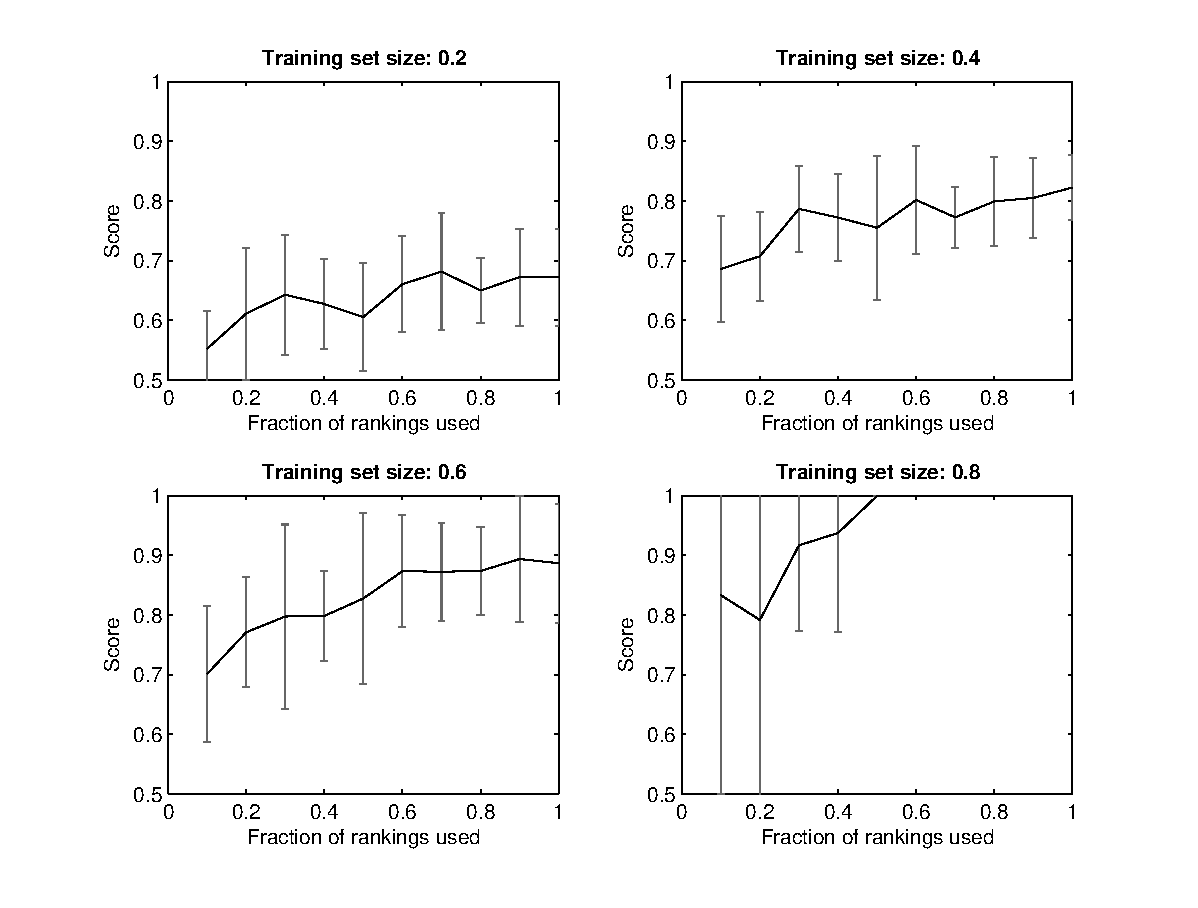
\includegraphics[width=1\linewidth]{rankings}
  \caption{Invloed fractie ongelijkheden}
  \label{fig:fractie}

\end{figure}

Figure~\ref{fig:fractie} shows how the scores improve as the amount of examples and the fraction of included inequalities increases.
In all cases more than half the pairs of examples are correctly predicted and high scores can be obtained even for small datasets.
Other experiments have shown that even for lower scores the optimization criteria are often capable of finding an optimal solution.

The underlying model can be directly expressed using the soft constraints that can be learned.
However, similar score are obtained for models which cannot be directly modeled, for example, the use of a weighted soft constraints which are disconnected.
While there are limits to the expressibility, the learned criteria are shown to be robust with respect to the exact formulation.

\begin{figure}

  \centering
    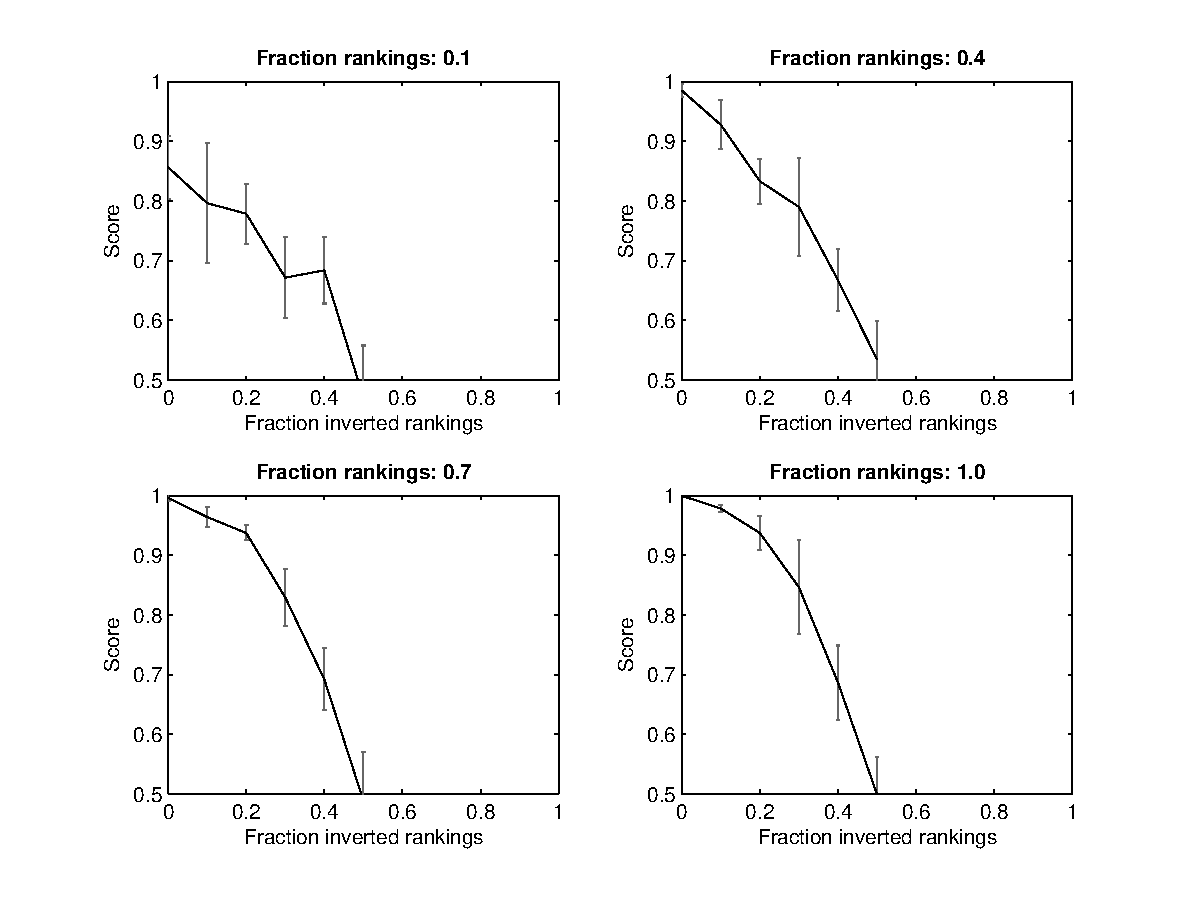
\includegraphics[width=1\linewidth]{noise}
  \caption{Invloed ruis}
  \label{fig:ruis}

\end{figure}

The influence of noise is shown in figure~\ref{fig:ruis}.
Hereby, the second approach of testing is used, where the all examples are used as test set.
The algorithm obtains high scores despite significant levels of noise.
Figure~\ref{fig:ruis} also shows that providing more rankings improves the robustness of the algorithm, even is the relative amount of noise remains unchanged.
Using the first approach with a training set of 40\%, scores over 0.7 can be obtained for noise levels of 20\%.

  \begin{table}
    \caption{Scores voor verschillende limieten ($t$)}
    \begin{tabularx}{\linewidth}{XXXX}
      $t = 1$ & $t = 2$ & $t = 3$ & $t = 4$ \\
      \toprule
     0.823 & 0.740 & 0.788 & 0.735 \\
     ($\pm$ 0.073)&
($\pm$ 0.078)&
($\pm$ 0.074)&
($\pm$ 0.063)
    \end{tabularx}
    \label{tbl:limiet}
  \end{table}

Finally, table~\ref{tbl:limiet} shows that increasing the threshold used for finding soft constraints does not improve the score.
This experiment used a 40\% training set and 40\% of the available rankings.
However, if the size of the problem and examples is increased, higher threshold will likely be appropriate.

\section{Conclusion}
The research in this thesis has focused on solving two problems: 1) learning constraints and 2) learning optimization criteria.
Implementation for both clause learning and clausal optimization have been provided that accomplish these tasks using first order logic clauses.

The constraint learning system has been able to learn the relevant hard and soft constraints in all experiments.
Herewith, the first goal of this thesis has been accomplished.
All problems have been solved in limited time (less than a minute), often even in a few seconds.
For each problem only a small number of examples was given to learn from.
The system requires only minimal information from the user.
However, it also allows the use of expressive background knowledge.
The learned constraints are domain independent, which facilitates the devise of positive examples.

The second goal of this thesis, learning optimization criteria, has been accomplished as well.
Optimization criteria are discovered that enable an optimal solution to be found.
Even for small datasets and noise on the rankings, constraints are found that enable most examples to be ranked correctly.

Aside from learning formal representations automatically from examples, this research shows how these representations can be used in practice.
This also forms an important step to enable the learning of optimization criteria in an interactive setting.

\paragraph{Future work}
This research offers multiple opportunities for future work.
It would be interesting to adapt the number of variables and literals in a clause dynamically.
This could be accomplished, for example, by using negative examples.
Learned clauses must be specific enough to not cover any negative examples. 

It would be interesting to add interactivity to the learning system, for the generation of examples or rankings.
Rankings expressing that examples are equally ranked are currently ignored.
However, it could be interesting to incorporate this information into the algorithm, whenever it is provided explicitly.

As mentioned earlier the domain independence of the clauses has several advantages.
In some cases, however, specific objects inherently present in the problem.
The constraint learning system could be enhanced to include such global constants.

\section*{Acknowledgments}
The author thanks his promoters Prof. dr. Luc De Raedt en Dr. ir. Anton Dries.
Furthermore, he expresses his gratitude for the help provided by Bart Bogaerts, Prof. dr. Jesse Davis, Prof. dr. Marc Denecker and Vladimir Dzyuba.
\\\\
{\color{red} References incorrect}

%
% ---- Bibliography ----
%
\begin{thebibliography}{}
%
\bibitem[1980]{2clar:eke}
Clarke, F., Ekeland, I.:
Nonlinear oscillations and
boundary-value problems for Hamiltonian systems.
Arch. Rat. Mech. Anal. 78, 315--333 (1982)

\bibitem[1981]{2clar:eke:2}
Clarke, F., Ekeland, I.:
Solutions p\'{e}riodiques, du
p\'{e}riode donn\'{e}e, des \'{e}quations hamiltoniennes.
Note CRAS Paris 287, 1013--1015 (1978)

\bibitem[1982]{2mich:tar}
Michalek, R., Tarantello, G.:
Subharmonic solutions with prescribed minimal
period for nonautonomous Hamiltonian systems.
J. Diff. Eq. 72, 28--55 (1988)

\bibitem[1983]{2tar}
Tarantello, G.:
Subharmonic solutions for Hamiltonian
systems via a $\bbbz_{p}$ pseudoindex theory.
Annali di Matematica Pura (to appear)

\bibitem[1985]{2rab}
Rabinowitz, P.:
On subharmonic solutions of a Hamiltonian system.
Comm. Pure Appl. Math. 33, 609--633 (1980)

\end{thebibliography}
\end{document}
